\documentclass[10pt, compress]{beamer}

\usetheme{m}

\usepackage{booktabs}
\usepackage[scale=2]{ccicons}
\usepackage{minted}

\usemintedstyle{trac}

\title{AngleGators}
\subtitle{A Game for the XO Laptops to help teach Angles}
\date{\today}
\author{Alexandria Mack - Melody Kelly - William Russel}
\institute{}

\begin{document}

\maketitle

\section{What is it?}

\begin{frame}{What is it?}
\begin{center}A game to teach angles to students at a fourth grade math level\end{center}
\end{frame}
    
    \begin{frame}{What is it?}
    \textbf{AngleGators}
    \begin{itemize}
    \item You are an alligator eating fruit as flows down the river.
    \item You need to open the alligator's mouth wide enough to eat fruit.
    \item The closer the alligator's mouth angle is to the the minimum fruit angle, the more points you get.
    \item Missing a fruit makes the Alligator lose a tooth
    \end{itemize}
    \end{frame}

\section{The Game}

\begin{frame}{The Game}
    \centering
    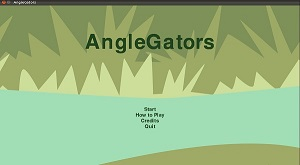
\includegraphics{images/home.jpg}
\end{frame}

\begin{frame}{The Game}
\centering
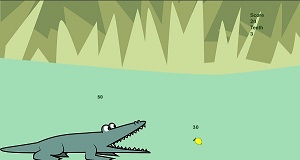
\includegraphics{images/Game.jpg}
\end{frame}

\section{How Does the Code Work}

\begin{frame}{How Does the Code Work}

\textbf{Awesome Things}
\begin{itemize}
\item \href{https://github.com/amm4108/AngleGators/blob/master/Scene.py}{The Menu System}
\item \href{https://github.com/amm4108/AngleGators/blob/master/Scene.py\#L140}{Highlighting of Clickable Items}
\item \href{https://github.com/amm4108/AngleGators/blob/master/angle_gators.py\#L104}{Returning Item Text to Decide What's Next}
\end{itemize}

\end{frame}

\begin{frame}{How Does the Code Work}

\textbf{Bad Things}
\begin{itemize}
\item \href{https://github.com/amm4108/AngleGators/blob/master/Alligator.py\#L48}{Alligator "Animation"}
\item \href{https://github.com/amm4108/AngleGators/blob/master/Food.py\#L63}{Food Draw Function}
\item \href{https://github.com/amm4108/AngleGators/issues/32}{No Sounds}
\item Game scores don't reset after 'Restart'
\end{itemize}

\end{frame}

\section{Stumbling Blocks and Successes}

\begin{frame}{Stumbling Blocks and Successes}
    \textbf Stumbling Blocks
    \begin{itemize}
    \item Setting the right item sizes and positions
    \item Showing the final score on the Game Over Screen
    \item Updating How Many Teeth are Left
    \item Getting the game running with a VM
    \end{itemize}
\end{frame}

\begin{frame}{Stumbling Blocks and Successes}
    \textbf Successes
    \begin{itemize}
    \item Semi Finished Game
    \item Functions Great on the XO
    \item Code is broken down well
    \item Score and lives work
    \end{itemize}
\end{frame}

\section{Things Done Differently}

\begin{frame}{Things Done Differently}
    \begin{itemize}
    \item Organized the code from the beginning
    \item Test frame rate difference from XO to other computers
    \item Test game on multiple operating systems, was only tested and working on Ubuntu and SugarOS
    \end{itemize}
\end{frame}

\section{More Time?}

\begin{frame}{More Time}
    \textbf{\href{https://github.com/amm4108/AngleGators/issues?q=is\%3Aopen+is\%3Aissue+milestone\%3A\%22Future+Things\%22}{Future Things}}
    \begin{itemize}
    \item Difficulty Levels
    \item Alligator Movement
    \item Make Screen Resizable
    \item Visually Lose a Tooth
    \item Game Music and Event Sounds
    \item Food Speed Variability
    \end{itemize}
    
\end{frame}

\begin{frame}{Wiki}
    \item \href{https://en.wikipedia.org/wiki/AngleGators}{AngleGators on Wikipedia.} 
    \item Will migrate wiki to SugarLabs

\end{frame}
\centering
\begin{frame}{Summary}

  Get the source of this theme and the demo presentation from

  \begin{center}\url{github.com/matze/mtheme}\end{center}

  The theme \emph{itself} is licensed under a
  \href{http://creativecommons.org/licenses/by-sa/4.0/}{Creative Commons
  Attribution-ShareAlike 4.0 International License}.

  \begin{center}\ccbysa\end{center}

\end{frame}

\plain{}{Questions?}

\end{document}
